\documentclass{article}
\usepackage[utf8]{inputenc}
\usepackage[margin=1in]{geometry}
\usepackage[spanish]{babel}
\usepackage{amsmath}
\setlength{\parskip}{1em}

\usepackage{xcolor}
\usepackage{listings}
\usepackage{xparse}
\NewDocumentCommand{\codeword}{v}{%
\texttt{\textcolor{blue}{#1}}%
}
\lstset{language=python,keywordstyle={\bfseries \color{blue}}}

\usepackage{graphicx}
\graphicspath{ {./images/} }


\title{Proyecto 1 - Física Computacional I}
\author{Camilo Gómez Zapata}
\date{Octubre, 2021}

\begin{document}

\maketitle

\section{Introducción}

Se desear estudiar numéricamente las soluciones propias de la ecuación de Schrödinger en una dimensión que tiene esta forma:

\begin{equation}
    -\frac{h^2}{2m}\frac{\partial^2\psi(z)}{\partial z^2}+V(z)\psi(z)=E_n\psi(z)    
\end{equation}

Con un potencial que puede tener varias formas, la principal de estas siendo la siguiente, que es la del pozo finito:

\begin{equation}
    V(z)= 
    \begin{cases}
       0 &|z|\leq a/2 \\
       V_0 &|z|> a/2
    \end{cases}
\end{equation}

Para esto se hallarán analíticamente los autovalores y autofunciones que satisfacen la ecuación, y después se observará el comportamiento de estos a través de gráficas.

\section{Desarrollo}

Lo primero que se procede a realizar es la solución analítica de este específico pozo de potencial, con sus correspondientes autovalores y autofunciones. Este problema ya ha sido estudiado ampliamente así que se revisarán los puntos más importantes de su solución. Después se aplica la solución analítica para resolver el problema computacional.

\subsection{Solución analítica del pozo de potencial finito}

Primero se divide el espacio en tres regiones, sean 1, 2, y 3, donde la 1 y la 3 corresponden a las regiones con el potencial $V_0$ y la 2 corresponde a la región intermedia. Así la solución está compuesta de 3 partes:

\begin{equation}
    \psi(z)= 
    \begin{cases}
       \psi_1 &z< -a/2 \\
       \psi_2 &-a/2\leq z\leq a/2 \\
       \psi_3 &z> a/2
    \end{cases}
\end{equation}

Teniendo el valor de $E-V_0$ donde $E$ es la energía total, se puede deducir que las soluciones tienen esta forma:

\begin{equation}
    \psi_1=Ge^{\alpha x}
\end{equation}
\begin{equation}
    \psi_2=A\sin(kx)+B\cos(kx)
\end{equation}
\begin{equation}
    \psi_3=He^{-\alpha x}
\end{equation}

Aplicando condiciones de frontera (igualando primeras y segundas derivadas en $x=-a/2$ y $x=a/2$) se generan dos tipos de soluciones: las simétricas y las antisimétricas. En el caso de las simétricas se cumple que $A=0$ y que $G=H$ y se puede deducir esto:

\begin{equation}
    He^{-\alpha a/2}=B\cos(ka/2)
\end{equation}
\begin{equation}
    \alpha=k\tan(ka/2)
\end{equation}

Y para las antisimétricas se cumple que $B=0$ y que $G=-H$. Para este caso se puede deducir esto:

\begin{equation}
    He^{-\alpha a/2}=A\sin(ka/2)
\end{equation}
\begin{equation}
    \alpha=-k\cot(ka/2)
\end{equation}

De ahí se puede ver que es dentro de las $k$ y las $\alpha$ donde va a estar la cuantización. Por la forma de la ecuación, estas tienen esta forma:

\begin{equation}
    k=\frac{\sqrt{2mE}}{\hbar}
\end{equation}
\begin{equation}
    \alpha=\frac{\sqrt{2m(V_0-E)}}{\hbar}
\end{equation}

Y se pueden convertir en adimensionales haciendo $u=\alpha a/2$ y $v=ka/2$. También se define esto:

\begin{equation}
    u_0=\frac{ma^2V_0}{2\hbar^2}
\end{equation}

Así, se cumpliría esto:

\begin{equation}
    u^2+v^2=u_0^2
\end{equation}

Y para el caso simétrico y antisimétrico se puede deducir que se cumple:

\begin{equation}
    \sqrt{u_0^2-v^2}= 
    \begin{cases}
       v\tan v&(simetrico) \\
       -v\cot v&(antisimetrico)
    \end{cases}
\end{equation}

Los $u$ y $v$ que cumplen este conjunto de ecuaciones son los que cuantizan la energía y deben ser hallados resolviendo las ecuaciones trascendentales. Finalmente se pueden despejar los autovalores de la ecuación $(11)$ que son de la forma:

\begin{equation}
    E_n=\frac{2\hbar^2v_n^2}{ma^2}
\end{equation}

\subsection{Algoritmo y gráficas}

El algoritmo de solución consiste en usar la fórmula de los autovalores y las fórmulas de las autofunciones para hallar el valor numérico de los primeros cuatro autovalores y las primeras cuatro autofunciones, y con base en esto hacer toda la simulación numérica con las gráficas que se pide.

Para esto se define una clase \codeword{Analyser} que es la que maneja toda la lógica, y se instancia recibiendo de argumento la función del potecial. En específico estos son los pasos del código:

\subsubsection{Hallar los autovalores y autofunciones}

Este es el paso más complicado. Aquí lo que se hace es hallar los autovalores con las fórmulas y dejar las autofunciones definidas como métodos. Para hacer esto se usan las expresiones analíticas que se acaban de hallar. Un detalle es que también debería funcionar para el pozo de potencial infinito y el oscilador armónico, por lo que la función que hace este procesamiento tiene un condicional que evalúa el potencial con el que fue instanciada la clase \codeword{Analyser} y decide cuál fórmula de autovalores y autofunciones usar.

Cuando el potencial es del pozo finito se hace un paso extra, que es hallar los ceros de las ecuaciones trascendentales (15). Esto se hace con un paquete de Python llamado \codeword{scipy.optimize}. Para que hayan en total cuatro ceros (cuatro $v_n$) hay que elegir $u_0^2$ correctamente:

\begin{equation}
    u_0^2=30
\end{equation}

Todo se asume adimensional, con $a=1$, $m=1$, $\hbar=1$ y $G=1$. Se hallan los cuatro $v_n$ que son estos:

\begin{equation}
    v_1=1.33, v_2=2.64, v_3=3.91, v_4=5.09
\end{equation}

Y se hallan los cuatro autovalores en este caso:

\begin{equation}
    E_1=3.54,E_2=13.94, E_3=13.73, E_4=51.82
\end{equation}

\subsubsection{Graficar autofunciones}

Para este potencial se hacen las gráficas entre $z=-1$ y $z=1$, como se ve en la figura 1.

\begin{figure}
    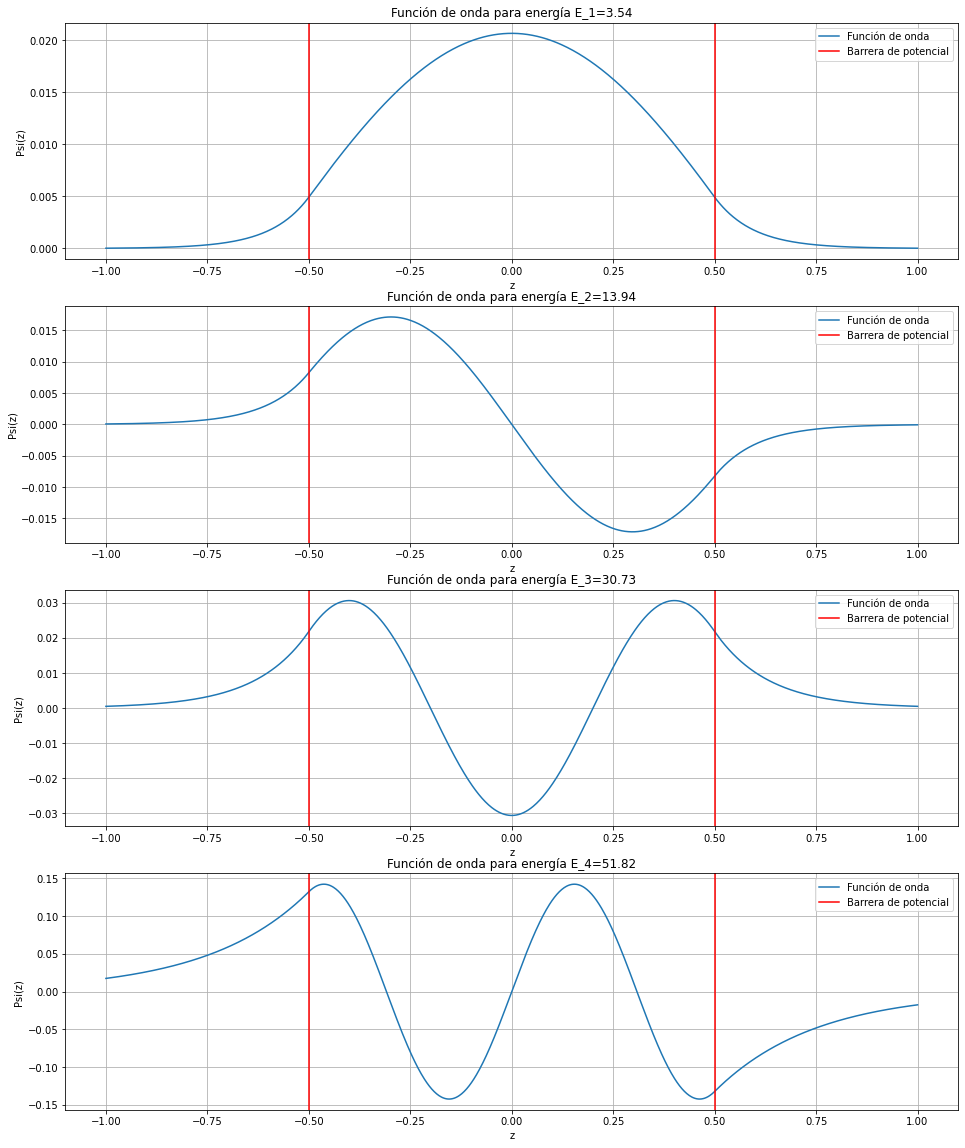
\includegraphics[scale=0.5]{images/fin_eigen.png}
    \centering
    \caption{Autofunciones para potencial finito.}
\end{figure}

\subsubsection{Graficar densidades de probabilidad}

Para todas las autofunciones encontradas se hacen las gráficas de densidad de probabilidad, que son tan solo las de las autofunciones elevadas al cuadrado, y se ven en la figura 2.

\begin{figure}
    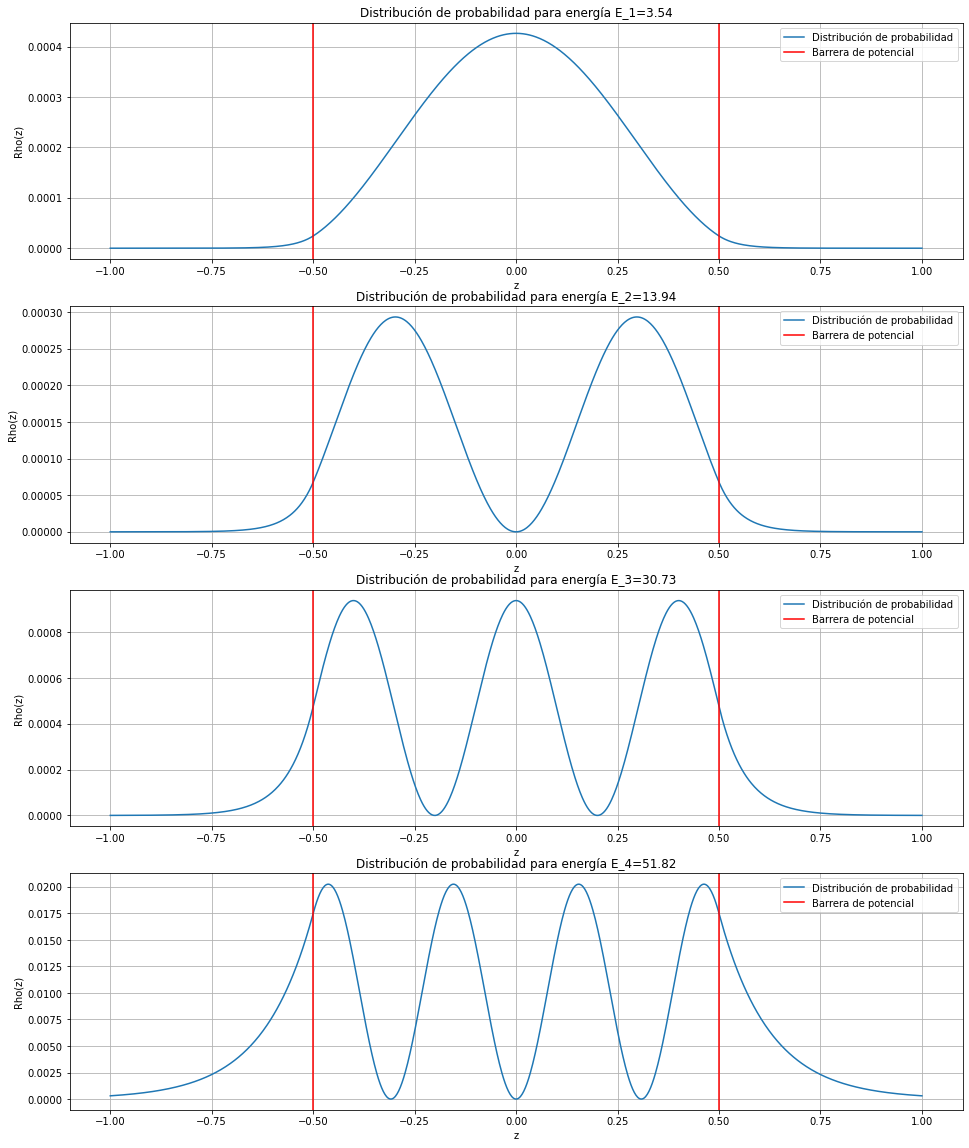
\includegraphics[scale=0.5]{images/fin_dens.png}
    \centering
    \caption{Densidades de probabilidad para potencial finito.}
\end{figure}

\subsubsection{Construir solución dependiente del tiempo y graficarla}

Se compone la solución dependiente del tiempo de esta forma:

\begin{equation}
    \Psi(z,t)=\sum_{n=1}^4c_n\psi(z)e^{-iE_nt/\hbar}
\end{equation}

Como son cuatro autofunciones, los coefiecientes $c_n$ que se eligen son $c_n=0.5$ para todo $n$, ya que esto cumple la condición de que la suma del cuadrado de los coeficientes sea 1. Se toman los tiempos $t=1s,2s,3s,4s$, como se ve en la figura 3.

\begin{figure}
    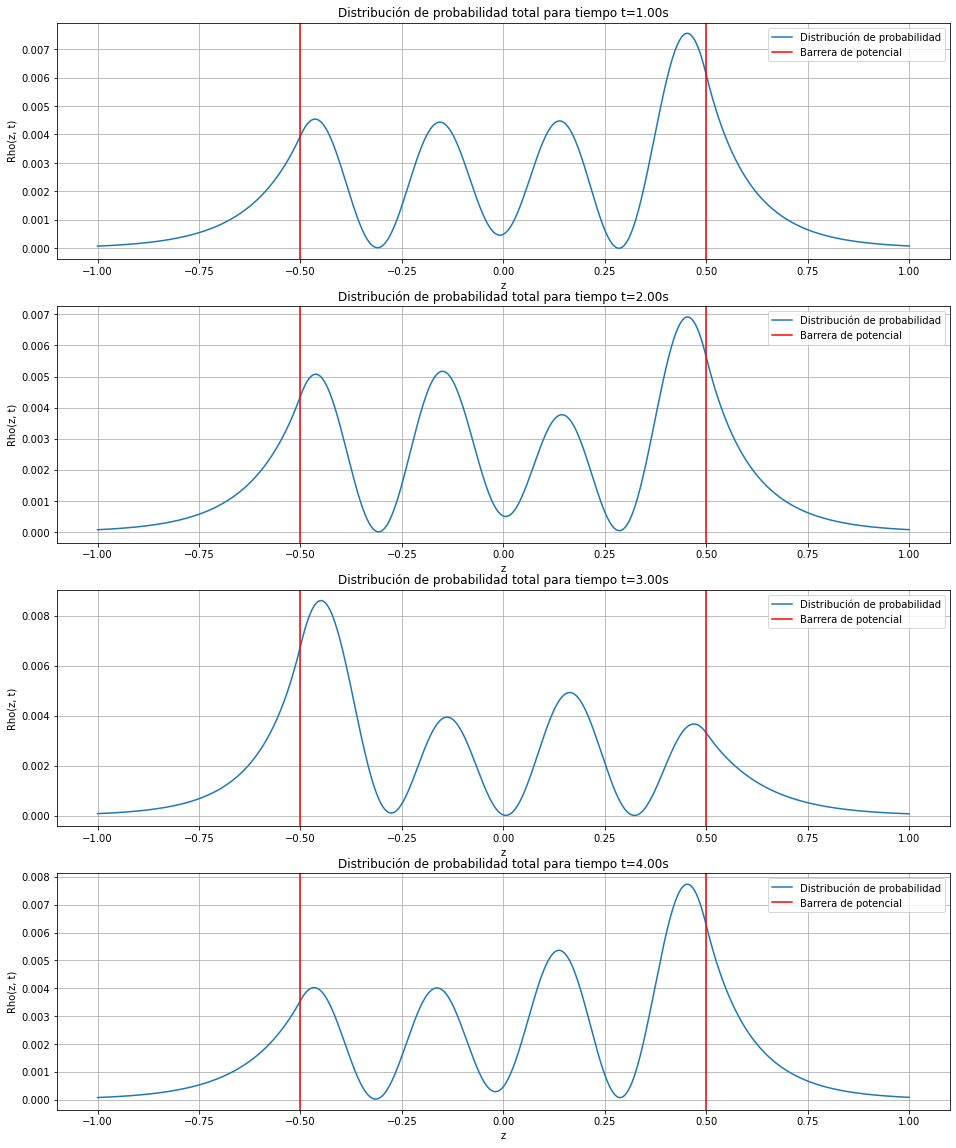
\includegraphics[scale=0.5]{images/fin_time.png}
    \centering
    \caption{Soluciones dependientes del tiempo para potencial finito.}
\end{figure}

\subsection{Pozo de potencial infinito}

Lo siguiente para hacer es repetir el mismo proceso pero para el pozo de potencial infinito. Este es más sencillo porque al ser infinito, la solución solo importa adentro y se desaparece en la frontera. Estos son los autovalores:

\begin{equation}
    E_n=\frac{n^2\pi^2\hbar^2}{2mL^2}
\end{equation}

Y las autofunciones:

\begin{equation}
    \psi_n(z)=
    \begin{cases}
       A\sin(k_n(x+a/2)) &|z|\leq a/2 \\
       0 &|z|> a/2
    \end{cases}
\end{equation}


Se realiza el mismo proceso para graficar las autofunciones (figura 4), las densidades de probabilidad (figura 5) y la solución dependiente del tiempo (figura 6). Se toma $A=1$.

\begin{figure}
    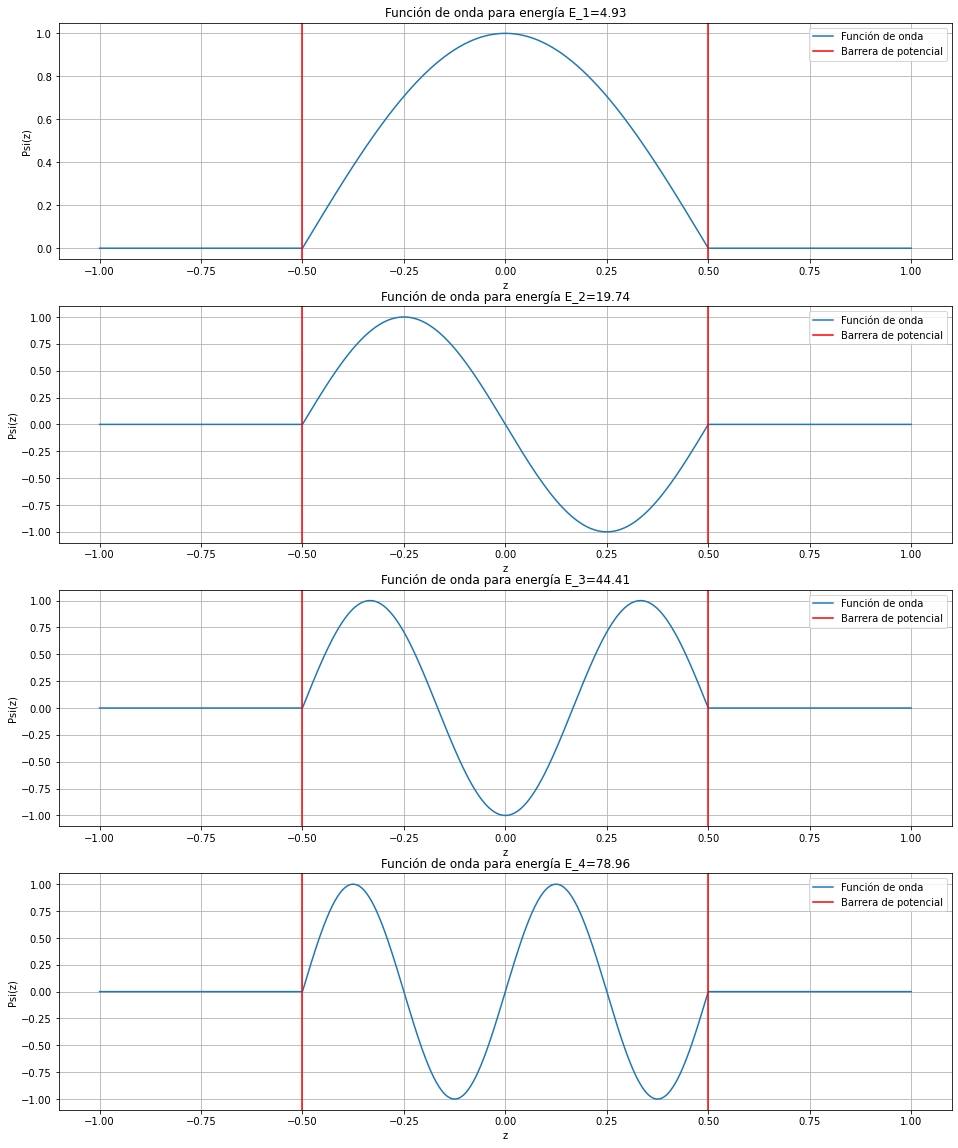
\includegraphics[scale=0.5]{images/inf_eigen.png}
    \centering
    \caption{Autofunciones para potencial infinito.}
\end{figure}

\begin{figure}
    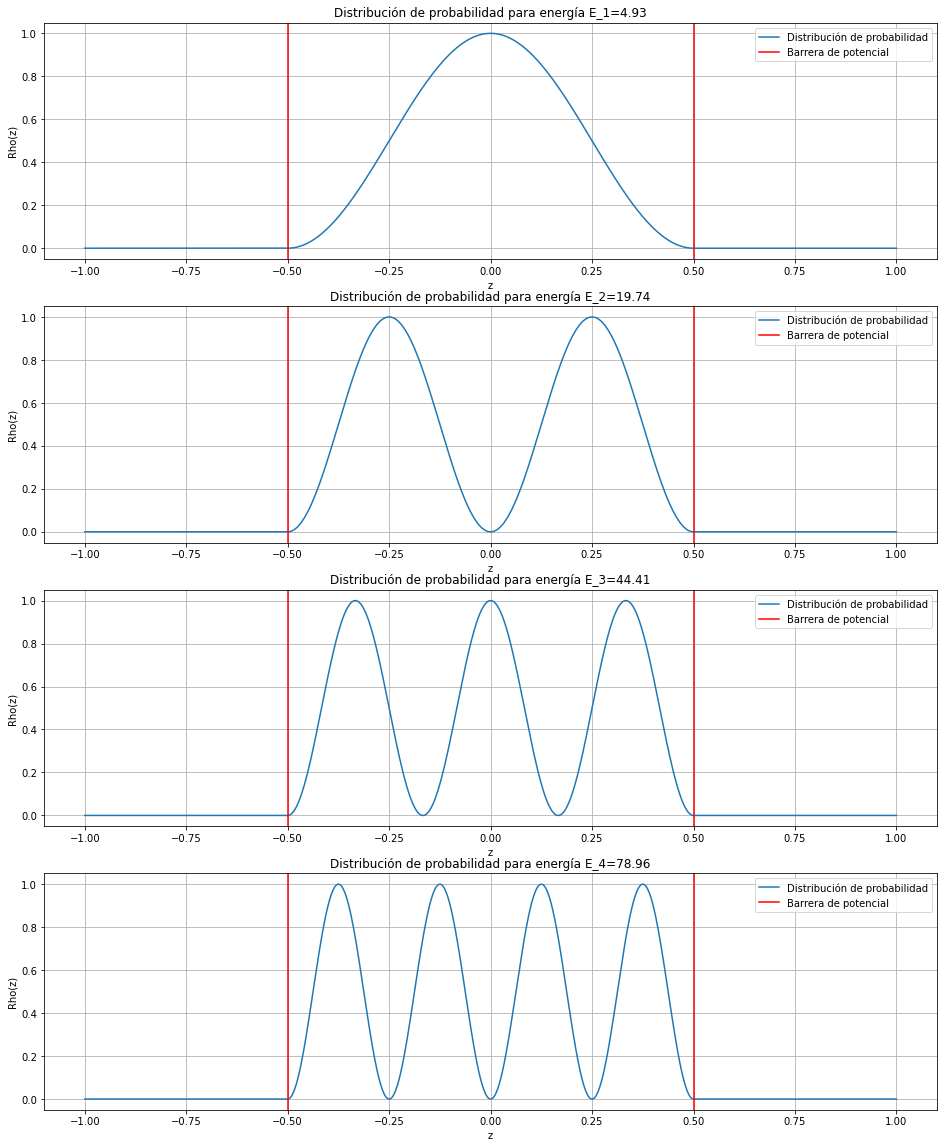
\includegraphics[scale=0.5]{images/inf_dens.png}
    \centering
    \caption{Densidades de probabilidad para potencial infinito.}
\end{figure}

\begin{figure}
    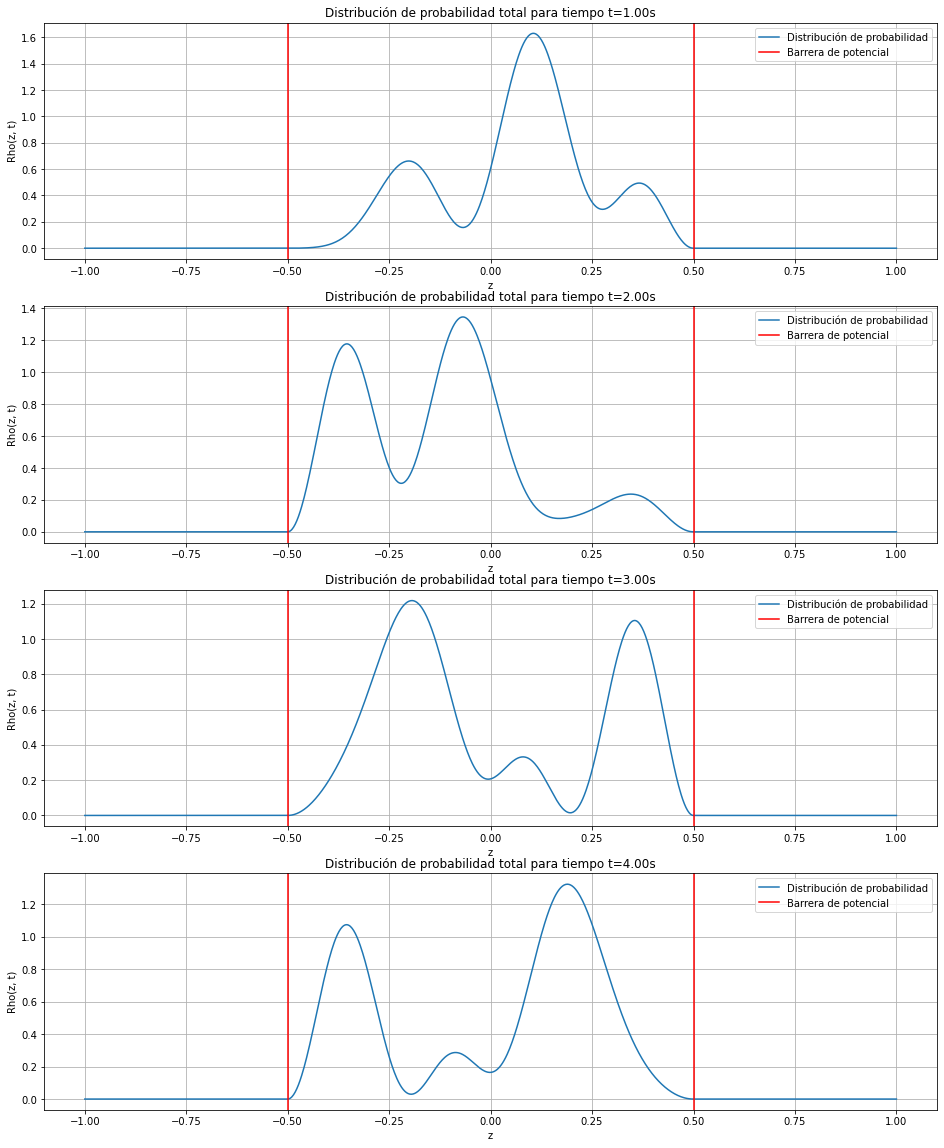
\includegraphics[scale=0.5]{images/inf_time.png}
    \centering
    \caption{Soluciones dependientes del tiempo para potencial infinito.}
\end{figure}

\subsection{Bono: oscilador armónico}

Aquí se usa el mismo código, nuevamente solo cambiando el potencial y sus autovalores y autofunciones correspondientes. Autovalores del oscilador armónico:

\begin{equation}
    E_n=\hbar\omega(n+\frac{1}{2})
\end{equation}

Y autofunciones del oscilador armónico:

\begin{equation}
    \psi_n(z)=\frac{1}{\sqrt{2^nn!}}\left(\frac{m\omega}{\pi\hbar}\right)^{1/4}e^{-\frac{m\omega x^2}{2\hbar}}H_n\left(\sqrt{\frac{m\omega}{\hbar}x}\right)
\end{equation}

donde $H_n$ son las funciones de Hermite, que se calculan con un paquete de Python llamado \codeword{scipy.special}. Se repiten las mismas gráficas de las autofunciones (figura 7) y las gráficas de las densidades de probabilidad (figura 8):

\begin{figure}
    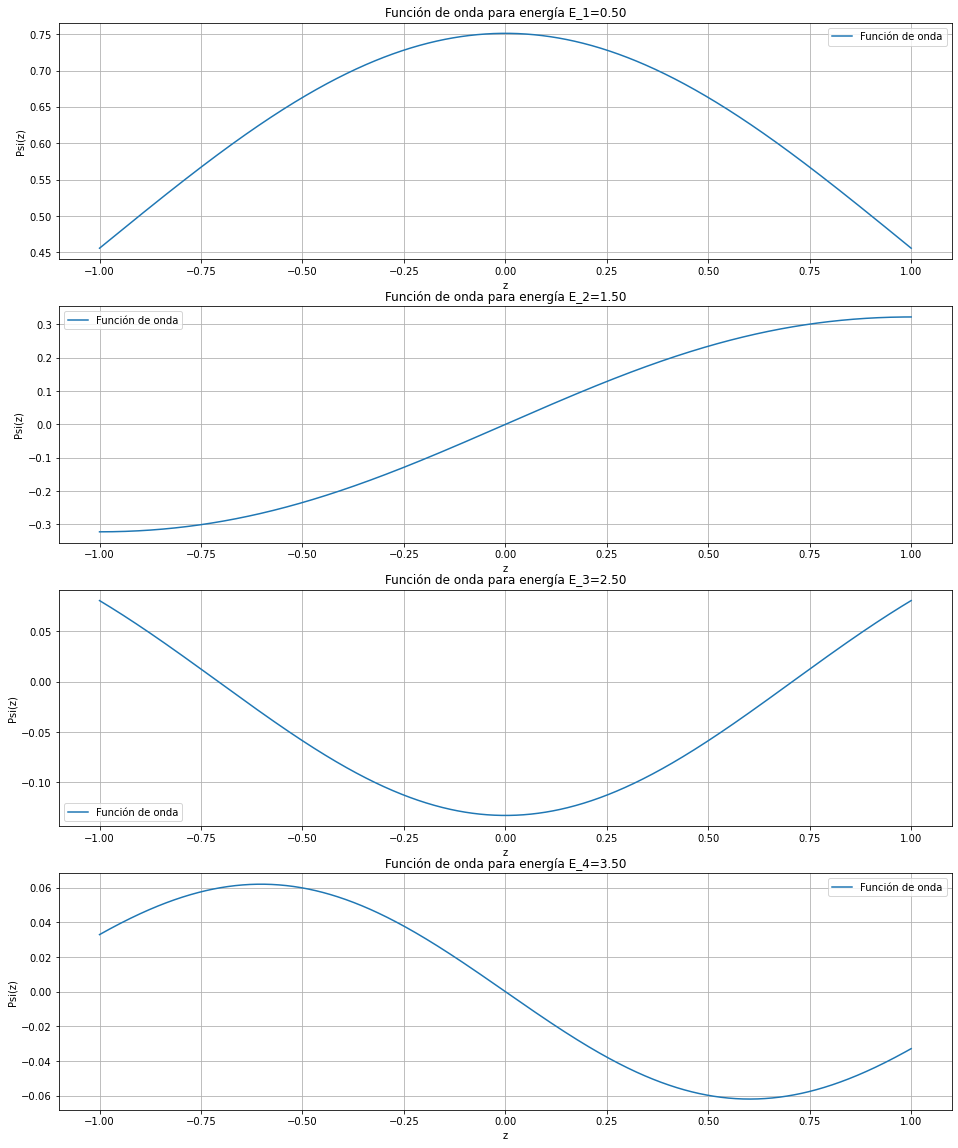
\includegraphics[scale=0.5]{images/harm_eigen.png}
    \centering
    \caption{Autofunciones para potencial armónico.}
\end{figure}

\begin{figure}
    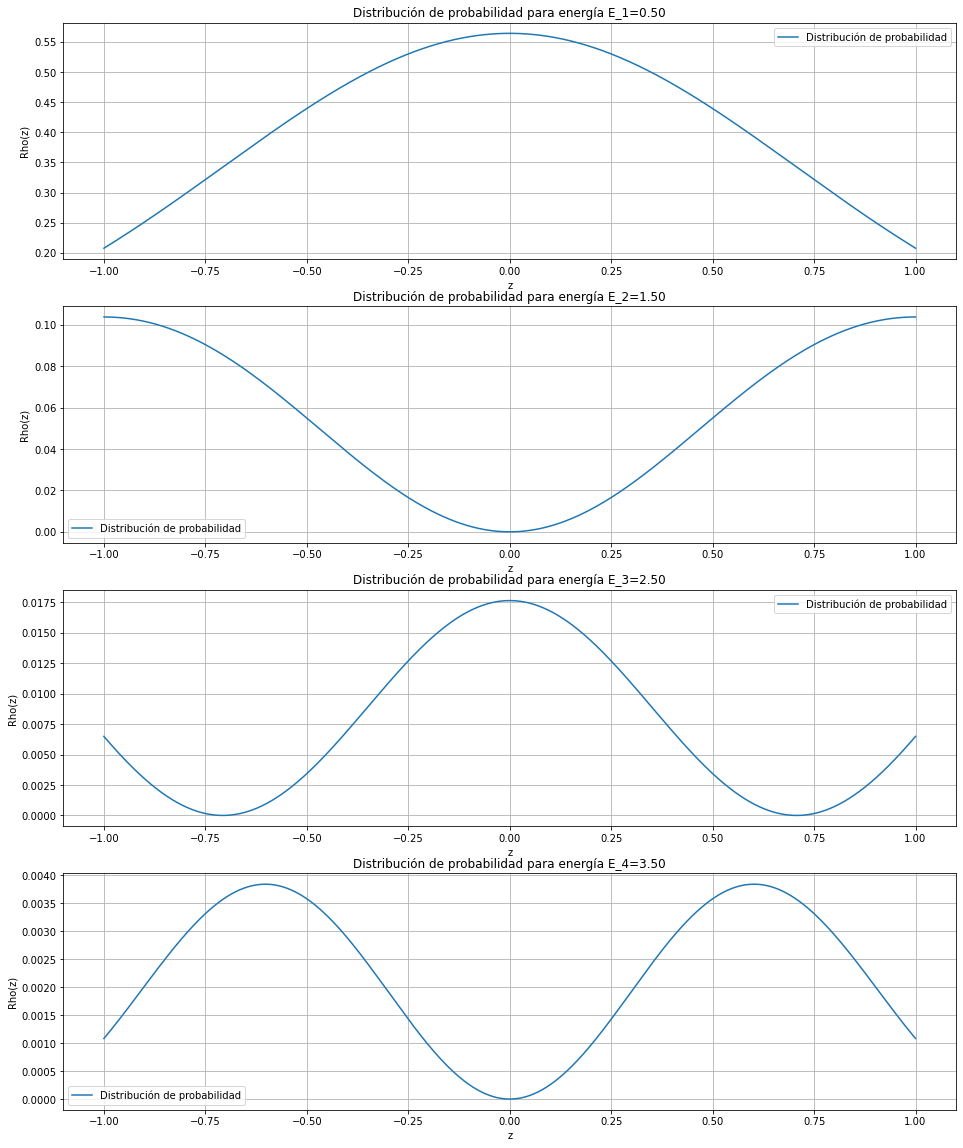
\includegraphics[scale=0.5]{images/harm_dens.png}
    \centering
    \caption{Densidades de probabilidad para potencial armónico.}
\end{figure}

\section{Conclusiones}

Con conocer los autovalores y las autofunciones correspondientes a una ecuación diferencial con un potencial dado, se tiene todo lo necesario para observar el comportamiento de los diferentes niveles de energía del sistema. Las gráficas con las diferentes energías son interesantes porque muestran el patrón armónico que suele seguir la función de onda, siempre bien comportada en las fronteras.

Un posible futuro paso, para mejorar la visualización, sería hacer una animación de cómo evoluciona el sistema en el tiempo, en vez de solo gráficas. Esto permitiría ver el comportamiento de estos niveles de energía de una forma mucha más detallada.


\section{Referencias}

- Particle in a box, Wikipedia. [https://en.wikipedia.org/wiki/Particle\_in\_a\_box]

- Quantum harmonic oscillator, Wikipedia. [https://en.wikipedia.org/wiki/Quantum\_harmonic\_oscillator]

- Finite potential well, Wikipedia. [https://en.wikipedia.org/wiki/Finite\_potential\_well]


\end{document}